
\documentclass[a4paper, 10pt, conference]{ieeeconf}
\overrideIEEEmargins

\title{\LARGE \bf
Report for Lab0 - Introduction to ROS\_ros
}

\usepackage{float}
\usepackage{url}
\usepackage{eurosym}
\usepackage{cite}
\usepackage[pdftex]{graphicx}


\author{Rodrigo Caye Daudt}


\begin{document}


\maketitle
\thispagestyle{empty}
\pagestyle{empty}


%%%%%%%%%%%%%%%%%%%%%%%%%%%%%%%%%%%%%%%%%%%%%%%%%%%%%%%%%%%%%%%%%%%%%%%%%%%%%%%%
\section{INTRODUCTION}

This report describes the work done for the practical work 0 (lab0) for the Probabilistic Robotics subject. The focus of this practice was to familiarize the students with basic concepts and tools in the Robot Operating System (ROS).


\section{OBJECTIVES}

The main objective of this work was to gather information about the turtlesim package and to develop a node in Python that controlled the movement of the turtle in the simulator so that it moved towards a chosen goal point in an appropriate manner. Therefore, the node would have to deal with ROS messages to read the current state (position and orientation) of the turtle and with the mathematics that would generate the control signal that would guide the turtle to the desired destination.


\section{METHODS AND RESULTS}

The first step to have any kind of closed loop control over the simulated turtle was to access its position and orientation. The turtlesim\_node publishes the spacial information of the turtle on a topic called turtle1/pose. The messages published on this topic were of the type turtlesim/Pose, which contained five variables regarding the position and velocity of the turtle. For this work, three of these variables were used: x, y, and theta.

Once we had access to the position of the turtle, it was necessary to know how to transmit the control signals to the turtle inside the simulator. This communication was done through a topic called turtle1/cmd\_vel, where messages of type geometry\_msgs/Twist could be published. On the Twsit object that was published, the parameter Twist.linear.x was used to control the linear velocity of the turtle and the parameter Twist.angular.z was used to control the angular velocity of the turtle inside the simulation.

To generate the control signals on this closed loop control system was to find the difference between the desired position and the current position. This numbers would determine the total distance to the goal, the angle to the goal and, consequently, the difference between the current angle of the turtle and the angle to the goal. These values were then fed into our control equations to obtain adequate linear and angular velocities that would be sent to the turtle.

One issue that was faced during the development of this controller was the range of the calculated value for the difference between the current angle and the desired angle. This value had to be put in the range $-\Pi \leq \Theta_{diff} < \Pi$ in order to make the turtle turn to the side which would lead to the fastest turn. $\Theta_{diff}$ was called $dt$ in the python code, and this operation can be found in line 92 of the turtle\_waypoint.py file.

Finally, to generate the control signals for the desired linear and angular velocities, PD controllers were used. The PD controller provided a solution with a very fast response and with high precision, while being stable for any goal and any initial state. It was observed that, although it would be a very small addition to the code, an integral channel to this controller would lead to oscillatory and perhaps unstable behaviour while adding nothing to the performance, since null steady state error for the static goals could be achieved even with a simple proportional controller. The parameters for both PD controllers (one for linear velocity and one for angular velocity) were tuned empirically. These parameters in the code had the names of kp\_v, kd\_v, kp\_w, and kd\_w, and can be found in lines 70-73 of the turtle\_waypoint.py file.

One final step that was taken in order to improve the results of the turtle simulation was to take into account the angle difference to control the linear velocity. The value calculated by the PD controller was multiplied by a factor of $cos(\Theta_{diff}/2)$ so that when the turtle pointed away from the target its linear velocity would be reduced, decreasing the amount of movement of the turtle away from the target and consequently decreasing the time it took to arrive at the goal position.

Figures \ref{traj11}, \ref{traj155}, and \ref{traj1010} show the trajectories taken by the turtle to reach different goals from the starting configuration (position $(5.5,5.5)$, $\Theta = 0$). In Fig. \ref{traj11} it is clear that the cosine regularization improves the results. We can see that since the target is directly behind the turtle, the first control signal tells the turtle only to turn (zero linear velocity), and it starts to move towards the goal on the second cycle (after 0.3 seconds) when the turtle is facing a direction roughly towards the goal.



\begin{figure}
   \centering
   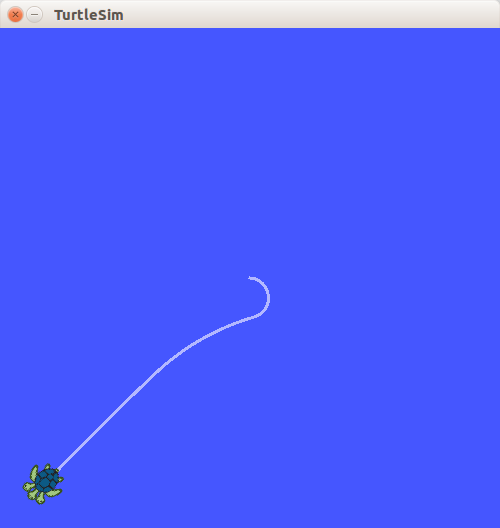
\includegraphics[width=2.5in]{figures/1-1.png}
   \caption{Trajectory of turtle from initial state to point (1,1)}
   \label{traj11}
\end{figure}
   
\begin{figure}
   \centering
   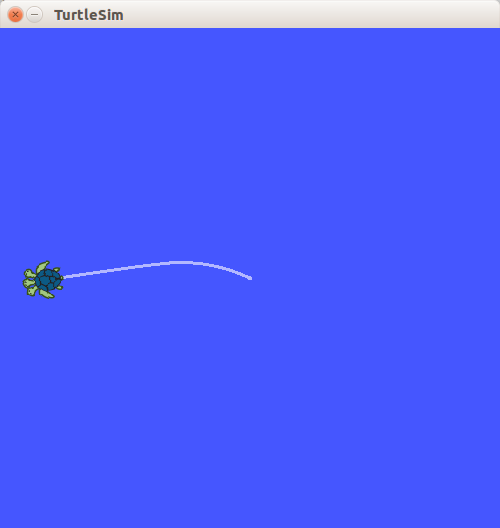
\includegraphics[width=2.5in]{figures/1-55.png}
   \caption{Trajectory of turtle from initial state to point (1,5.5)}
   \label{traj155}
\end{figure}
   
\begin{figure}
   \centering
   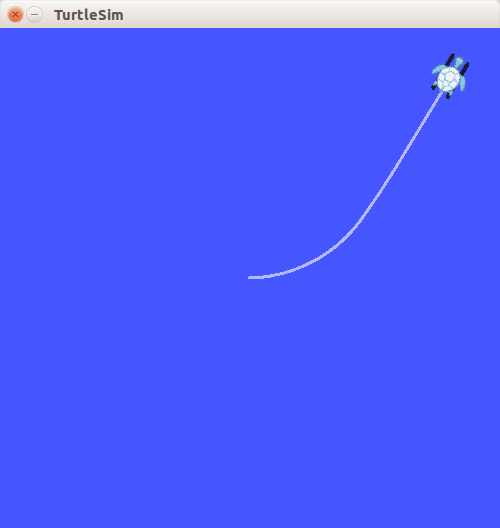
\includegraphics[width=2.5in]{figures/10-10.png}
   \caption{Trajectory of turtle from initial state to point (10,10)}
   \label{traj1010}
\end{figure}

%%%%%%%%%%%%%%%%%%%%%%%%%%%%%%%%%%%%%%%%%%%%%%%%%%%%%%%%%%%%%%%%%%%%%%%%%%%%%%%%
\section{DISCUSSION AND CONCLUSIONS}

The control system developed here provided a fast and precise solution to the control of the turtle, while using few lines of code and being computationally inexpensive. It illustrates basic techniques of linear control by using PD controllers to control two variables (linear velocity and angular velocity) which are not completely independent. An extra step was added to the control system to improve the way the control was done by taking into account how these variables interacted. This practice also served the purpose of teaching and solidifying the knowledge of basic principles of operation of various aspects of the ROS environment.




\begin{thebibliography}{99}

\bibitem{c1}
Lab0 - Introduction to ROS, Probabilistic Robotics.

\bibitem{c2}
turtlesim/Pose Documentation, \url{http://docs.ros.org/indigo/api/turtlesim/html/msg/Pose.html}

\bibitem{c3}
geometry\_msgs/Twist Documentation, \url{http://docs.ros.org/api/geometry_msgs/html/msg/Twist.html}


\end{thebibliography}

\end{document}
